%%%%%%%%%%%%%%%%%%%%%%%%%%%%%%%%%%%%%%%%%
% Journal Article
% LaTeX Template
% Version 1.3 (9/9/13)
%
% This template has been downloaded from:
% http://www.LaTeXTemplates.com
%
% Original author:
% Frits Wenneker (http://www.howtotex.com)
%
% License:
% CC BY-NC-SA 3.0 (http://creativecommons.org/licenses/by-nc-sa/3.0/)
%
%%%%%%%%%%%%%%%%%%%%%%%%%%%%%%%%%%%%%%%%%

%----------------------------------------------------------------------------------------
%	PACKAGES AND OTHER DOCUMENT CONFIGURATIONS
%----------------------------------------------------------------------------------------

\documentclass{article}

\usepackage{lipsum} % Package to generate dummy text throughout this template

\usepackage[sc]{mathpazo} % Use the Palatino font
\usepackage[T1]{fontenc} % Use 8-bit encoding that has 256 glyphs
\linespread{1.05} % Line spacing - Palatino needs more space between lines
\usepackage{microtype} % Slightly tweak font spacing for aesthetics

\usepackage[hmarginratio=1:1,top=32mm,columnsep=20pt]{geometry} % Document margins
\usepackage{multicol} % Used for the two-column layout of the document
\usepackage[hang, small,labelfont=bf,up,textfont=it,up]{caption} % Custom captions under/above floats in tables or figures
\usepackage{booktabs} % Horizontal rules in tables
\usepackage{float} % Required for tables and figures in the multi-column environment - they need to be placed in specific locations with the [H] (e.g. \begin{table}[H])
\usepackage{hyperref} % For hyperlinks in the PDF

\usepackage{lettrine} % The lettrine is the first enlarged letter at the beginning of the text
\usepackage{paralist} % Used for the compactitem environment which makes bullet points with less space between them

\usepackage{abstract} % Allows abstract customization
\renewcommand{\abstractnamefont}{\normalfont\bfseries} % Set the "Abstract" text to bold
\renewcommand{\abstracttextfont}{\normalfont\small\itshape} % Set the abstract itself to small italic text

\usepackage{titlesec} % Allows customization of titles
\renewcommand\thesection{\Roman{section}} % Roman numerals for the sections
\renewcommand\thesubsection{\Roman{subsection}} % Roman numerals for subsections
\titleformat{\section}[block]{\large\scshape\centering}{\thesection.}{1em}{} % Change the look of the section titles
\titleformat{\subsection}[block]{\small}{\thesubsection.}{1em}{} % Change the look of the section titles

\usepackage{graphicx}

\usepackage{fancyhdr} % Headers and footers
\pagestyle{fancy} % All pages have headers and footers
\fancyhead{} % Blank out the default header
\fancyfoot{} % Blank out the default footer
\fancyhead[C]{Bachelor Seminarium $\bullet$ TI3700 $\bullet$ Delft University of Technology} % Custom header text
\fancyfoot[RO,LE]{\thepage} % Custom footer text

%----------------------------------------------------------------------------------------
%	TITLE SECTION
%----------------------------------------------------------------------------------------

\title{\vspace{-15mm}\fontsize{18pt}{10pt}\selectfont\textbf{A comparison of supervised learning classifiers for oil spill detection}} % Article title

\author{
A.S.Y.Chiu \\ \scriptsize{[Andy's TU email]@student.tudelft.nl}  \and
     \and T.P.van Helden \\ \scriptsize{t.p.vanhelden@student.tudelft.nl}
   \and S.S.Jahanshahi\\ \scriptsize{S.S.Jahanshahi@student.tudelft.nl}
}

\date{}

%----------------------------------------------------------------------------------------

\begin{document}

\maketitle % Insert title

\thispagestyle{fancy} % All pages have headers and footers

%----------------------------------------------------------------------------------------
%	ABSTRACT
%----------------------------------------------------------------------------------------

\begin{abstract}

  Marine oil spills cause big problems, financially and ecologically. To prevent and react accordingly to oil spills, detection is required. This detection process is not easy and successful discrimination of oil spills and lookalikes(e.g. algae, grease ice, rain cells and low wind areas) is dependent on the classification techniques used. This is why different classifiers are studied that support the decisions of experts in an automatic detection system. In this paper we look specifically at the classification of oil spills in Synthetic Aperture Radar (SAR) images. We compare three commonly used classifiers: Support Vector Machines (SVM), Decision Trees (DT) and MultiLayer Perceptrons (MLP) based on their accuracy and overall characteristics in order to give a recommendation. A wide range of papers using the different classifiers is discussed and their performance compared. It is hard and inappropriate to directly compare classifiers in terms of accuracy since they all use different datasets and different features. MLP is often used in oil spill detection and increasingly in the more broad area of remote sensing. MLP and SVM are well suited when large number of labelled samples are available because of their ability to handle non-linear data, but they are prone to over fitting. The more easy to understand DT should be considered when data is scarce. We recommend that the oil spill community creates a shared database. Also, further research on bagging and image fusion to increase the availability of data in this field should be done. Random Forests and SVM require more attention of the oil spill detection community, as they seem to be interesting candidates for the classification of oil spills.


\end{abstract}

%----------------------------------------------------------------------------------------
%	ARTICLE CONTENTS
%----------------------------------------------------------------------------------------

\begin{multicols}{2} % Two-column layout throughout the main article text

\section{Introduction}

  Marine oil Spill is a form of human made environmental pollution usually occur during transportation of oil, drilling platforms or tankers \cite{Zhang201476}or during the maintenance on oil exploration sites in the ocean. One of the largest occurrences of oil spills in the history happened in the Gulf of Mexico as the oil spread out in the ocean by the explosion on the drilling platform affected marine ecosystem and wild life\cite{Bozeman2011244}.\\
Detection of oil spills can help to control environmental risks and prevent incalculable damages by it. Synthetic aperture radar(SAR) image is useful to detect oil spills spots in the ocean. \\
There are various automated systems proposed in order to detect spills spots in SAR images. These systems analyzes the SAR images, assigns the probability of dark spots and proposes an algorithm to classify the dark images in to the oil spills and look alike shapes \cite{Xu201414,brekke2008classifiers,Keramitsoglou2006640,Guo2014146}.\\
We will start this article by looking at different system for detecting oil spills, but we will focus on SAR. Afterwards, we will examine the preprocessing of SAR images. Thirdly, an explanation of the features used in oil spill detection is given. We shortly touch on how they are extracted and why these are commonly used. We then quickly explain the three different supervised learning classification methods we want to compare. In section four we compare our three classifiers with each other. We then have a discussion based on the results of section four. Here we look at which classifier is a good choice for oil spill detection. We finalize our paper with a conclusion.

%------------------------------------------------

\section{Oil spill detection methods}

	Oil spill detection can be done with several methods. In the field of optical imaging alone, there are plenty of options. Aircrafts can create images across various spectra of light with different cameras. After heating, oil emits certain levels of infra red radiation. Another method is to measure the reflectance, since oil reflects light differently than water. Laser fluorsensors measure the emission fluorescent light when oil hit by ultraviolet light. But all these methods have a several downsides as well. Though reflectance is higher in oil, it does not show a distinct pattern in reflecting light \cite{fingas2014review}. This makes it hard to distinguish between oil and other reflective surfaces. Also, this technique can only be applied when there is light. Infra red techniques requires heat to function.
SAR has a high resolution, wide area coverage and moreover images can be taken day and night under any weather condition. This enables oil spill investigators to monitor oceans 24 hours a day\cite{Chang20081915}. The advantage of this is that large areas can be checked for spills, which is often required when checking oceans. 
The main alternative within radar imaging is Side-Looking Airborne Radar(SLAR), which is an older but significantly cheaper method \cite{fingas2014review}. 

SAR images are created through radio waves. Radio waves are sent from the SAR device to an area. That area reflects radio waves in a certain way, which is measured through the time the waves take to travel back  \cite{Doerry:04}. When an ocean is hit by radio waves, those waves are reflected in a certain way. Oil reflects radio waves in a different way. This difference is the key to identifying oil spills.
In the image that is drawn from these measurements, water is shown as a grey or lighter area, while oil is shown as a dark spot. 









\section{SAR preprocessing}

	There are many factors that can cause problems in SAR images. An overview is presented in figure \ref{fig:overview}.
\begin{figure}[H]
	\centering
    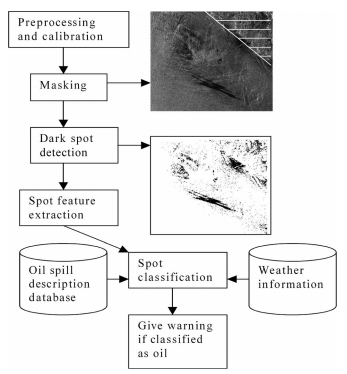
\includegraphics[width=50mm,scale=0.3]{./img/detection_diagram.png}
    \caption{\footnotesize{Overview for the oil spill detection approach \cite{Solberg200745}}}
    \label{fig:overview}
\end{figure}
Preprocessing the SAR image is done to improve the contrast between dark spots and the water surrounding them, as well as flag certain dark spots to be ignored. 

First, there is a general quality assessment. If the image is blurred in general, it will be impossible to get any information out of it. Afterwards, experts look at noise removal. One of the most common versions of noise is speckle noise. Speckle noise is caused naturally by a disruption in the phase of radio waves. Radio waves leave the sensor all in the same phase. Once they interact with an object, they scatter and are out of phase with each other. If they interact with each other, the result will be a darker or lighter pixel than it should. Multi-look processing and spatial filtering can be done to reduce speckle noise \cite{simard1998analysis}.

Experts also flag (mask) areas in the image which might interfere with the classification process. These areas include shorelines, land and ships, as these would all be represented by dark areas in the images. Land masses are usually identified using GPS and marked with Geographical Information System \cite{star1990geographic}. These systems allow for the storing, analyzing and manipulation of maps and images using geographical information. Ships can be identified if their route or position is known. A problems arises when the information is not public or missing in some way.
Another possibility is that dark spots are caused by algae or seaweed infestations \cite{fingas2014review}. These can be masked if, for instance, local ecological experts have knowledge of these formations. Grease ice, rain cells and passing unknown vessels can all be mistaken for oil spills \cite{Brekke200595} so they need to be filtered out. The problem is that it is hard to filter out every dark spot, since there is so much information and some critical information might not be public or present.

These preprocessing steps will make classification easier, but is still a difficult task. In some cases a human expert can't even tell the difference \cite{Keramitsoglou2006640}. Through image segmentation, all dark spots are taken in isolation and the values of predefined features are extracted from them. Classification can now be performed by using the features as input where the output of the chosen classifier will be the probability of the dark spot being an oil spill or a lookalike. %THIS PART NEEDS A REFERENCE 
High or low wind areas are also taken into consideration as they change the surface of the water and oil slicks. This in turn could have influenced the reflection of radio waves and in turn the image \cite{fingas2014review}.

In an automated detection system, a high oil spill probability can lead to a warning message.




\section{Features}
	
	In order to classify dark spots as either oil spills or lookalikes, features are extracted from them to calculate the probability for the two possible outcomes. A feature is an identified measurable property concerning the dark spot and which value has a strong statistical relationship with the classification output. Around 25 features are commonly used for oil spill classification and can be found in the table below. %\ref{fig:featuretable}

\begin{minipage}[H]{0.28\linewidth} % A minipage that covers half the page 
\footnotesize
\tabcolsep=0.09cm
\centering
\begin{tabular}{{|l|ll|l|}}
	\toprule[1.5pt]
  \textbf{No} & \textbf{type} & \textbf{Features} & \textbf{Code} \\
    \hline
    1 & \textbf{Geometrical} & Area & A \\
    2 & & Perimeter & P \\
    3 & & Perimeter to area & ratio P/A \\
    4 & & Complexity & C \\
    5 & & Shape factor I & SP1 \\
    6 & & Shape factor II & SP2 \\
    7 & \textbf{Physical} & Object mean value & OMe \\
    8 & & Object standard deviation & OSd \\
    9 & & Object power to mean ratio & Opm \\
    10 & & Background mean value & BMe \\
    11 & & Background standard deviation & BSd \\
    12 & & Background power to mean ratio & Bpm \\
    13 & & Ratio of the power to mean ratios & Opm/Bpm \\
    14 & & Mean contrast & ConMe \\
    15 & & Max contrast & ConMax \\
    16 & & Mean contrast ratio & ConRaMe \\
    17 & & Standard deviationcontrast ratio &  ConRaSd \\
    18 & & Local area contrast ratio & ConLa \\
    19 & & Mean border gradient & GMe \\
    20 & & Standard deviation border gradient & GSd \\
    21 & & Max border gradient & GMax \\
    22 & & Mean Difference to Neighbors & NDm \\
    23 & \textbf{Textural} & Spectral texture & TSp \\
    24 & & Shape texture & TSh \\
    25 & & Mean Haralick texture & THm \\
    \bottomrule[1.5pt]
\end{tabular}
%\caption{The 25 most commonly used features\cite{Topouzelis201268}}
\label{fig:featuretable}
\vspace{2cm}
\end{minipage}

The features can be divided into three major categories\cite{Brekke200595}:
\begin{enumerate}
\item (1 - 6) geometric characteristics (e.g. area, perimeter, complexity)
\item (7 - 22)Physical characteristics of the backscatter level of the spot and its surroundings (e.g. mean, max backscatter value)
\item (23 - 25) Texture (e.g. mean contrast)
\end{enumerate}

Geometric characteristics are the features that are related to the shape of the dark spot and is applied by all methods in the table\cite{Topouzelis200930}. An important feature is how elongated a spot is, which is expressed as a ratio between the width and length of the dark spot\cite{Gasull20071}. A study has shown that oil spills can be discriminated according to their shape\cite{Guo2014146}. The majority of oil spills have a linear shape that is either straight or angular\cite{Pavlakis200156}. Features that use the backscatter level of the spot and its surroundings take into account the gradient level in the image. For example, the background standard deviation is a feature that is highly effected by wind level and is generally high for lookalikes. Texture provides information about the spatial correlation among neighbouring pixels. Contextual features are not included in the table, but are considered very useful\cite{Topouzelis200930}. They incorporate other information not all extractable from the image, but is available as prior knowledge. These include the distance between a dark spot and a ship, weather information, distance to shore and whether the dark spot lies in a frequently polluted area. Most classifiers rely heavily on geometric shape features and the contextual feature.\cite{Xu201414}

Researchers have tried to reduce the amount of features to counter the curse of dimensionality which makes the dataset become more sparse as the dimensionality increases. Training a classifier with a sparse dataset will have lower predictive power. Fewer features also reduce the risk of over fitting, which is what happens when the classifier is too trained on specific data instead of capturing the underlying relationship. This leads to poor generalization of the data and thus has an negative impact on the classification process.

Features belonging to the same category appear to be highly correlated \cite{Xu201414}, leading to the search for a subset of features with less redundancy and retains most of the predictive power. How many and which features to include is known as the feature selection problem. Including too many features leads to a larger geometric space requiring the classifier to be more complex. Important information is lost when leaving too many features out, researchers try to find the right balance. The resulting subset will allow shorter training times and reduce over fitting. The values of these features are calculated and used as inputs in a chosen classifier.


%------------------------------------------------

\section{Classifier summary}

\subsection{What is supervised learning}

	Machine learning corresponds to the study and construction of systems that can learn from data. These systems can be useful when typical rule based programs that follow explicit instructions do not give good performance. Their ability to learn makes them popular in the field of artificial intelligence and pattern recognition. Machine learning can take several forms. In this paper, we look specifically at classifiers within the field of supervised learning. In supervised learning the system is trained or `taught' using input data that is known to belong to a certain class of output.\\ 
%A mapping between the inputs and outputs is inferred from the training data which can be used to classify unseen data. \cite{cord2008machine}

For the purpose of understanding how supervised learning works, consider a supervised learning model that is shown in fig \ref{fig:SL}. First step is to normalize raw data and prepare data for the training set and validation set. Next data is randomly allocated to these two sets (usually 60\% for the training set and the rest for validation set). The training set is used by classifier to learn how to classify the data. The training data will feed into the algorithm in order to learn from training data so that it designs a model that wishes to predict an unseen data. When the model is built, validation set analyzes the model by testing its accuracy. It is important in this stage to use data that are not used by the model before, this is why in the second step of figure \ref{fig:SL} the data is split into two.  If a validation set gives out an error rate larger than the training set, then we have to go back, tweak the model and adjust the parameters. Since the build model has already seen the training data, and has memorized the answer, is not trustworthy anymore. As a consequence, the model tries to `memorize' the data instead of `learning' to generalizes. This will make generalization properties of the model, to become progressively worse and is known as over-fitting or over-training\cite{wiki:of} problem in machine learning. However, depending on the type of a classifier, there are techniques to avoid this problem, e.g. to avoid over-fitting in neural network training\cite{Piotrowski201397}. The moment that model shows consistency, it can be used to predict and label an unknown data. \\  
 
\begin{figure}[H]
\centering
    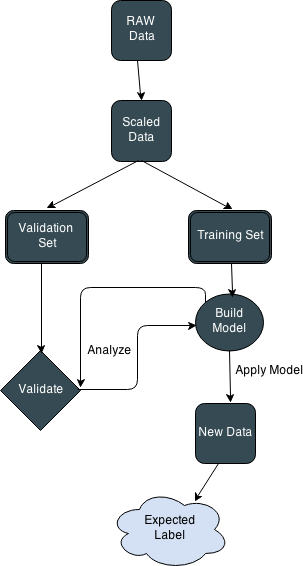
\includegraphics[width=38mm,scale=0.3]{./img/SL.png}
    \caption{\footnotesize{An overview of Supervised learning model that divides scaled data into two sets in order to build a model and predict unseen data }}
    \label{fig:SL}
\end{figure}

In unsupervised learning, no associated label, which is the desired output for a set of inputs, is given to the learning algorithm. The class belonging to each instance in the dataset is unknown and there is no reward when the classifier picks the right class. This technique is therefore more often used when trying to discover hidden classes in new datasets \cite{maglogiannis2007emerging}.








\subsection{Support Vector Machines}

	
Support Vector Machines(SVMs) is a classifier which outputs an optimal hyperplane or set of hyperplanes in high-dimensional space and classifies new examples(unseen data). In other words, SVMs are supervised learning models that employs learning algorithms to recognize patterns and analyze data, used for classification of unknown data\cite{wiki:SVM}.\\
In figure \ref{fig:SVM} main idea behind SVMs is shown. Consider example dataset described by variables $x_1$ and $x_2$. The operation of SVM algorithm is based on finding the optimal hyperplane between training examples. An optimal hyperplane is the one that gives largest minimum distance to the training examples and It maximizes the margin of training data\cite{opencv_library}.

\begin{figure}[H]
    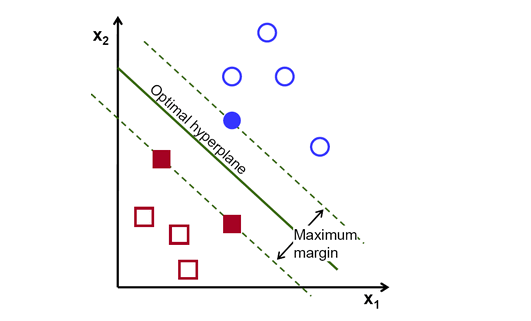
\includegraphics[width=80mm]{./img/SVM.png}
     \caption{Optimal Separating Hyperplane}
    \label{fig:SVM}
\end{figure}

In recent years, SVMs are widely used in bio-informatics \cite{furey2000support,osuna1997training,guyon2002gene} and other discipline due to its ability to accurately deal with high dimensional data\cite{joachims1998text}. They are popular for couple of theoretical reasons: SVMs are robust to very large number of variables and can learn both simple and complex classification models\cite{cristianini2000}.\\

SVMs is a best known member in the general category of kernel methods\cite{shawe2004kernel}. A kernel method has the ability to generate non-linear decision boundaries by using method designed for linear classifiers; This allows the user to apply a classifier to data that has infinite- dimensional vector space representation such as DNA or protein\cite{ben2010user}.    






\subsection{Decision trees}

	A decision tree is a classifier that makes several sequential decisions. The outcome of that sequence determines whether a data point belongs to one class or another. The structure of a decision tree \ref{fig:DT} is defined as a set of nodes ${x_1, ... , x_n}$ with edges ${e_1, .., e_{m}}$ between them. The edges are directed and there are no cycles in the network. The tree has one root $x_1$. With each data point we start at the root. The root node is fed information about a certain feature. The root node then evaluates a rule or function that allows the node to make a decision about what class a data point probably belongs to. Each decision leads to a different node, where another decision is made, increasing the likelihood that the data point belongs to a certain class. This process repeats itself until one of the leaf nodes is reached \cite{safavian1991survey}. From there we can determine what class our initial data point belonged to (either class $A$, $B$ or $C$ in the figure below. 

\begin{figure}[H]
    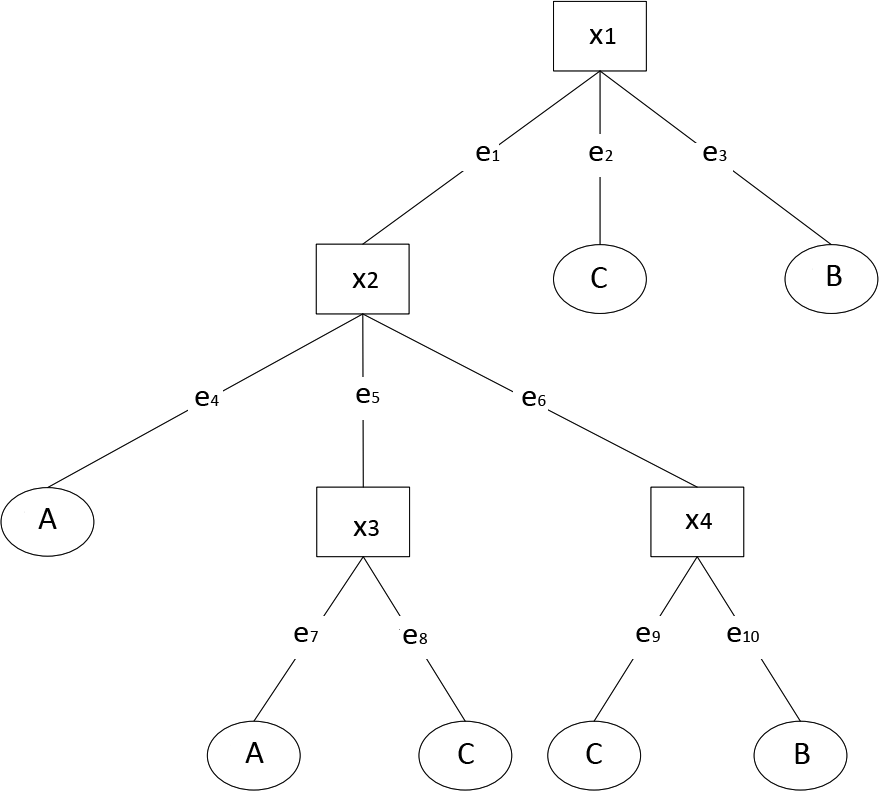
\includegraphics[width=80mm]{./img/decisiontree.png}
    \caption{\footnotesize{Decision Tree example. $x_i$ are nodes where decisions are made. $e_j$ are edges leading down the tree to other nodes. $A,B,C$ are classes that instances are to be classified into.}}
    \label{fig:DT}
\end{figure}

Decision trees are generally built or `grown' with a simple algorithm. Of course random selection of features is an option, but there are many other approaches, like the famous ID3 \cite{quinlan1986induction} and C4.5 algorithm \cite{quinlan1993c4}. ID3 roughly works as follows: We create a node that splits the tree into at least 2 branches. To create a node, we compare every feature and split the one with the highest information gain. In other words, the division will give us a lot of information about the data points and their classes. For example: in classifying trees and plants, height might give more information about which class an instance belongs to than the colour of its leaves would. For each of the subsets that comes forth out of that division, the process is repeated until there is enough certainty that the remaining subset represents the class. This does not take into account that a combination of features might make for an even better split, but it is a relatively efficient algorithm. %Another example of a tree building algorithm is called Fisher's Linear Discriminant Tree \cite{LópezChau20136283}. Fisher's tree is based on maximizing the distance between the means of classes. 

A tree stops to grow when the impurity level is low enough. The impurity level is a metric to indicate what the chances are of misclassification. A simple example for any $node_j$ would be $impurity(node_j) = 1 - max(P(z_i = c_a) $. Here $z_i$ is the $i^{th}$ instance of the subset at our node to be classified into class $c_a$. 

The opposite of growing a tree is called `pruning'. This is done to decrease the complexity of the tree and reduce chance of over fitting. The experts may decide to prune a tree as well if, in hindsight, the training data was faulty in some way. Pruning is done by removing the least significant node(s). 

It is also possible to combine multiple decision trees into a Random Forest \cite{breiman2001random}. This allows for higher accuracy as well as handling higher complexity. Features to split the trees are chosen randomly for each tree. To have enough samples to train the forest, bagging can be performed. Bagging takes random samples from a dataset, with replacement. With this, you have more smaller dataset (with duplicates) that you can train on. With enough trees, the variance of the accuracy decreases. Within forests, every instance to be classified is classified by every tree. The class of an instance is determined by majority vote over all the trees. 

In general, the more nodes a tree has, the more accurate it can be trained. The downside is that the time to classify and train will increase the larger the tree becomes, as well as an increased risk in over fitting. The design of the tree is crucial, as each node splits up the dataset in a certain way. Dividing a datasets in the wrong order can make for significantly slower and less accurate trees. The advantage of the decision tree is it's computational efficiency \cite{safavian1991survey}, its intuitive structure and resistance to noise \cite{LópezChau20136283}.

\subsection{Multi Layer Perceptrons}

	\hspace{0.5cm} MultiLayer Perceptrons are a type of supervised learning \cite{michie1994machine}. It is a type of neural network consisting of multiple layers of perceptrons. A perceptron is a system of nodes with input nodes, called the input layer, and an output node called the output layer. Inputs from a vector $x$ are fed to the input layer with weights $w$. Within the perceptron, each input value is compared with a certain function and increased by a certain weight. The output is determined based on the threshold
\begin{figure}[h!]
  \caption{Rosenblatt's perceptron}
  \centering
    
\includegraphics[width=55mm]{./img/perceptron.png}
    \label{fig:perceptron}
\end{figure}

%------------------------------------------------

\section{Comparison of classifiers}

\subsection{SVM Vs DT}

	It is impossible to fully compare Support Vector Machines and Decision Trees. Both have advantages and disadvantages, each serving it's own purpose. One such difference is that DTs are faster when handling new datasets, compared to SVM. This is because of the complexity of SVMs' arithmetic computations, where DTs only need to follow a logical path in a tree. A more interesting difference is that SVM has higher accuracy in general as was observed in numerous studies\cite{arun2010hybrid}.
 
A study more closely related to SAR used hydro acoustics to classify different species of fish. Sonar is used to create hydro acoustic images, which results in similar images as SAR \cite{griffiths2003synthetic}. Fourteen features were used. Both SVM and DT were considered good classifiers. SVM required more preprocessing time, but had slightly higher results. DT was easier to implement and easier to read. However, DT showed greater variance \cite{Robotham2011170}.

SVM and DTs were also compared in a study using LandSat images. They used SVM, DT and Maximum Likelihood Classifier (MLC) to determine different types of land coverage (e.g. forest, water, wetlands, open grasland) in Uganda. Though the spatial dimension of LandSat (which produces optical/visual images) is lower than the average SAR satellite, there are a lot of similarities. Out of eight classes, both SVM and DT were able to distinguish seven classes. DT had a slightly higher accuracy rate and higher kappa statistic \cite{Otukei2010S27}.





\subsection{SVM Vs MLP}
	
	SVM and MLP are two known classifiers that has lots of potential to truthfully predict classification solutions. According to Wolpert and Macready, in their paper\cite{wolpert1995no}, they have indicated that `any two optimization algorithms are equivalent when their performance is averaged across all possible problems'. This makes it difficult to choose a supreme classifier.  Researchers\cite{Moavenian20103088,Zanaty2012177} has practiced some experiments to know which classifier might predict more accurate than other; the outcome of this experiments indicated that SVM outperforms MLP in one case while In another type of dataset SVM falls below MLP. If a comparison is done theoretically then SVM and MLP has their own distinguishing advantages. SVM classifiers has a strong founding theory and need less memory to store the predictive model; Even when training sample has some bias, If the right parameters are chosen for SVM, then it can be robust\cite{auria2008support} but advantages of MLP are not as few as SVM. MLPs are popular in machine learning solutions such as speech recognition, image recognition because of their ability to solve problems stochastically, meaning that it allows user to get approximate solution for very complex problems like fitness approximation\cite{jin2005neural}. Here we will look closely at SVM and MLP performance using real world dataset in various disciplines(ECG arrhythmias,text recognition, remote sensing, wind speed prediction) to examine performance of them. It is obvious here that free lunch theorem\cite{wolpert1995no} is valid, sine there is no superior classifier to other in all cases!\\
In the field of ECG(Electrocardiography), comparison between MLP and SVM is done using same dataset. MLP accuracy in classifying the ECG(Electrocardiography) signals, is more accurate than other ANN. MLP with back propagation(BP) training algorithm suffer from slow convergence to local minima, on the other hand SVM classifier with (K-A) training do not trap in local minima points therefore they are faster than ANN\cite{Moavenian20103088}.\\
 In high dimensional data, SVM accomplishes better accuracy compare to MLP, this is when new kernel function proposed for SVM. The reason behind is that MLP needs more hidden units for tested data set and become more complex when the dimension of data set increases whereas SVM complexity does not depend on dimension of data set. SVM are efficient on optimal separation of unseen data points\cite{Zanaty2012177}.\\
SVM works better than MLP for the off-line signature recognition(within finite database). The comparison is done between the identification rate(increment of 20\% for SVM) and for training time needed. The superiority of SVM is because of its generalization ability in high dimensional space\cite{FriasMartinez2006693}.\\
SVM outperforms to MLP, in Wind speed prediction. The comparison is done using a wind speed dataset that cover a 12 years between 1970-1982. Dataset is divided into three parts: training, test and validation sets. The output result shown the SVM outperform MLP on all orders resulting in the lower MSE(MLP is 0.0090 while it is 0.0078)\cite{Mohandes2004939}.\\
In oil spill detection, the datasets are imbalanced, in which most instances(that are not oil spill spot) belong to a larger class and very few instances for smaller class(oil spill spot). Lack of instances in minority class will cause SVM suffer from biased decision boundary and prediction performance, however combining SVM with an over-sampling and under-sampling technique will make SVM outperform to other classifiers\cite{liu2006boosting}.

	
      




	

\subsection{DT Vs MLP}

	\begin{itemize}
	
	\item  In \cite{Mera2014} a Decision Support System to detect oil spills has been created. For classification both a neural network and a decision tree are used. Since both classifiers are designed and tested using the same data, a comparison on accuracy can be made. The neural network appears to outperform the decision tree slightly.\cite{Moavenian20103088}
	
	\item  Another study by \cite{Xu2014} also compared different classifers for oil spill detection. Here they experienced an opposite result. Out of seven classifiers, the ANN was found to perform the worst by 14.8 percentage points. The results indicated that the additional flexibility provided by SVM and ANN does not necessarily improve the predicitive performance compared to less flexible methods. Both tend to overfit the dataset on small-sized training samples and could not generalize well.
    

\end{itemize}



	

\section{Discussion}

	There are some key issues for effectively classifying dark spots, several factors should be taken into account \cite{Kubat:1998:MLD:288808.288812}. First of all, the available data containing oil spills is scarce compared to lookalikes. This leads to a very imbalanced dataset. As a consequence, a classifier sensitive to this problem can not reach it's maximum accuracy \cite{Japkowicz20026}. SVM seem the least affected by this imbalance. Second, there is no guarantee that the data used for training the classifier are representatives of future samples, especially with such scarce datasets as in oil spill detection. This issue is known as the validity of data. Furthermore, the feature selection procedure should be done with care as it can influence prediction accuracy. Out of the 25 common features, most researchers arbitrarily select a subset of features and compare multiple subsets using cross-validation, a technique for estimating how well a model generalizes to an independent dataset. Finally, a classifier should be chosen with all the issues mentioned in mind including ease of interpretation and training times in a highly dynamic environment. In the table \ref{fig:table}, all previously mentioned studies are shown including their results and characteristics. This should allow a better discussion on which classifier is well suited for oil spill detection.

\begin{table*}[t]

\advance\leftskip-3cm
\setstretch{1.5}
\tabcolsep=0.19cm
\small
\centering


%\adjustbox{max width=0.97\pdfpagewidth, left}{
\begin{adjustbox}{width=\textwidth,totalheight=\textheight,keepaspectratio}
\begin{tabular}{*{6}{|l|}}

\toprule[1.5pt]
  \textbf{Study} & \textbf{Data Type} & \textbf{Preprocessing} & \# \textbf{Features} & \textbf{Formations(lookalike \& oilspills)} & \textbf{Results} \\
    \hline
  
    Hydro-acoustics \cite{Robotham2011170} & Sonar & Echoview & 15 &  - & SVM accuracy: $89.5$\%, DT accuracy: $86.8$\% \\

    Land coverage1986 \cite{Otukei2010S27} & LandSat SAR & `Using data miner' & 11 &  - & SVM max accuracy: $90.53$\%, DT accuracy: $93.48$\% \\

    Land coverage2001 \cite{Otukei2010S27} & LandSat SAR & `Using data miner' & 10 &  - & SVM max accuracy: $93.67$\%, DT accuracy: $94.07$\% \\ 
    
    Oil spills\cite{Topouzelis200762} & ERS-2 SAR, 24 high-res images 8-bit & transformation, Filtering, data normalization & 10 & 90  \& 69  & MLP(10:51:2) accuracy: $86.67$\% lookalike acc. $91.18$\% oil spills acc.\\
    
    Oil spills\cite{Delfrate200038} & ERS SAR, 600 low-res images & Resampling,Radiometric range correction, georeference & 11 & 68  \& 71  & MLP(11-8-4-1) accuracy: $90$\% lookalike acc. $82$\% oil spills acc.\\
    
    Oil spills\cite{Topouzelis200930} &  ERS-2 SAR, 24 high-res images & - & 10 & 90 \& 69  & MLP(10-51-2) accuracy: $84.4$\% lookalike acc. $85.3$\% oil spills acc.\\
    
    Oil spills\cite{Topouzelis200924} &  ERS SAR, 12 high-res images & 8-bit transformation, filtering & - & - & MLP(4-2-1) accuracy: $96.46$\% overall acc. \\
 
    Oil spills\cite{Delfrate2004} &  ERS SAR, 70 images & - & 12 & 78 \& 111  & MLP(12-8-8-1) 0.227 root mean square error(rmse)\\
    
    Oil spills\cite{Xu201414} &  RADARSAT-1, 93 images & log-transformation, standardization & 15 & 94  \& 98  & MLP $75.93$\% overall acc. SVM $79.63$\% overall acc. DT(Bundling) 90.74 overall acc.\\
    
    Oil spills\cite{Mera201472} &  Envisat, 47 images & - & 9 & 155  \& 80  & MLP(9:11:2) $96.3$\% lookalike acc. $92.9$\% oil spill acc. \\
    & & & & & DT $92.6$\% lookalike acc. $92.9$\% oil spill acc. \\
    
    Oil spills\cite{Delfrate1996} &  ERS-1 SAR, 59 low-res images & - & 9 & 2471 \& 42  & DT $96$\% lookalike acc. $86$\% oil spill acc\\
    
    Oil spills\cite{Topouzelis201268} &  ERS-2 SAR, 24 high-res images & - & 9 & 90  \& 69  & DT forest $84.4$\%\\ 
    
    Oil spills\cite{brekke2008classifiers} & ENVISAT, 103 images & masking & - & 12244 \& 41  & SVM(C-SVC) $77.4$\% lookalike acc. $82.9$\% oil spill acc.\\

    ECG arrhythmias\cite{Moavenian20103088} & MIT-BIH arrhythmia database & - & 10 & - & accuracy SVM 99\% , MLP 98.22\% \\

    Remote Sensing\cite{Zanaty2012177} & Satimage & feature extraction & 26& - & accuracy for SVM 93.16\% ,and for MLP 96.98\%\\
    
    signature recognition\cite{FriasMartinez2006693} & user signature data &feature extraction& 2 & - & Recognition rate SVM 66.5  , MLP 71.2\\
    wind speed prediction\cite{Mohandes2004939}& daily wind speed data & - &high dimensional feature & - & MSE on testing data for the MLP is 0.0090 while it is 0.0078 for the SVM\\
    
    Hashimoto's disease\cite{Omiotek201340} &  66 Thyroid ultrasound images & normalization & 59 & 54 healthy and 85 sick & MLP(6-8-1): $89.4$\% sick class $61.1$\% healthy class. DT: $89.4$\% sick class $94.4$\% healthy class. \\
    
    \bottomrule[1.5pt]
    
\end{tabular}
\end{adjustbox}
\caption{\footnotesize{An Overview of oil spill and related studies with their results and charateristics}}
\label{fig:table}
\end{table*}

These studies reported varying results in accuracy. Studies not related to oil spills have shown similar performance. Accuracies up to 96\% are claimed\cite{Topouzelis200924}, but without even specifying the data used for training and testing, these results are highly questionable. When looking at the table\ref{fig:table}, it is hard and inappropriate to directly compare classifiers in terms of accuracy since they all use a different dataset. Researchers have tried to eliminate this issue by using the same dataset for each of the classifiers in a comparison\cite{Mera201472}\cite{Xu201414}. Even though classifiers are trained with the same data, the validity of data issue persists. Since real world samples are scarcely available, classifiers may be insufficiently trained to generalize the dataset. Much improvement in classifier comparisons can be achieved if researchers would have access to a common database\cite{Topouzelis200810}.
An emphasis exists on the minimization of false negatives for detecting oil spills. In an automatic decision support system where many images are analyzed, an oil spill classified as a lookalike will have higher environmental consequences. Another factor that has an impact on accuracy are the selected features used as input to a classifier. Although in most cases a similar amount of features is used, only some are taken together in different studies. The search for an optimal set of features has been tried using a genetic algorithm \cite{Topouzelis200930}, but this may not exist.
MLP is often used in oil spill detection and increasingly in the more broad remote sensing as well. Their ability to simultaneously handle non-linear data of a multi-dimensional input space is a large advantage. Furthermore, they do not require an explicit well defined relationship between input and output as they determine the relationship on their own using training set data. This ability to learn is why MLP are considered reliable classifiers and useful for oil spill detection \cite{Delfrate200038}. Surprisingly, decision trees achieve a similar performance compared to the more complex SVM and MLP. This can be attributed to the fact that decision trees perform better when dealing with categorical features and that SVM and MLP require a large dataset to achieve its maximum prediction accuracy \cite{kotsiantis2007supervised}. Apart from this, decision trees are easily understood. This intuitiveness is important because classification systems in oil spill detection usually serve as a decision support system. Decision trees are faster to train, but the classifiers are only trained once. When a large dataset is available, MLP and SVM are well suited for detecting oil spills, because they both perform well when a non-linear relationship exist between the input and output features \cite{kotsiantis2007supervised}. If training data is scarce however then decision trees can be considered since SVM and MLP are more prone to overfitting in oil spill detection\cite{Xu201414}.


\section{Conclusion}

	This paper presented a comparison between three popular classification techniques for the detection of oil spills using SAR images. Few papers employed decision trees or SVM which is why studies of similar problems that are related to oil spill detection have been included. Not all papers agreed on a particular classifier having the highest accuracy, but this could have been expected since the results are under discussion and direct comparison is difficult. Each experiment uses a different data set, some even included unverified samples. The chosen classifier largely depends on the complexity of the problem, feature dimension, type of features and the data set. Even for seemingly similar problems this can lead to the usage of a different classifier. SVM and MLP are recommended when the dataset is complex, because of their ability to handle non-linear classes. Single decision trees can be considered when training time and ease of interpretation matter, when data is scarce or when there is a lot of noise in the image. 

In the case of oil spill detection, much improvement in the research about different classifiers can be done by establishing a common database with labelled dark spots that are verified. Preferably, dark spots in all shapes, sizes and on different geographical points. This will allow researches to train a classifier with the same data set. Further research could include more data and a combination of classifiers.

To further increase the availability of data, we suggest more research is done on bagging. Sampling datasets multiple times can at least increase the amount of data available for training or validation purposes. Perhaps it can even help balance some datasets.

Another interesting option to increase data availability, is the fusion of images. This is done to fuse different types of data together, namely LandSat and SAR. Perhaps a similar technique can be used to extend SAR images. Again, this would not allow for new real data, but might help with training classifiers.

Finally, few studies use used Random Forests. These seem to give interesting results when used for classification of oil spills. They have some of the advantages of decision trees but can also handle more complex data. On the other hand, they might act more like a black box, losing the advantage of intuitiveness. This would be an interesting classifier to research.
	
\end{multicols}

\newpage
%----------------------------------------------------------------------------------------
%	REFERENCE LIST
%----------------------------------------------------------------------------------------

\bibliographystyle{plain}
\bibliography{references}
%----------------------------------------------------------------------------------------




\end{document}